\documentclass[14pt]{extarticle}
\usepackage{amsmath}
\usepackage{amssymb}
%\usepackage{tikz}
%\usetikzlibrary{calc}
%\usetikzlibrary{trees}
\usepackage{hyperref}
\usepackage{graphicx}
\graphicspath{ {../../chap09/} }
\usepackage[top=0.75in, bottom=0.75in, left=0.75in, right=0.75in]{geometry}
%\newcommand*{\Scale}[2][4]{\scalebox{#1}{\ensuremath{#2}}}%
\usepackage[shortlabels]{enumitem}
\usepackage[most]{tcolorbox}
\definecolor{bg}{RGB}{255,249,227}
% \usepackage{showframe}
\title{\vspace{-5ex}Math 208 Section 9.2}
\date{\vspace{-10ex}}
%\usepackage{multicol}
%\setlength{\columnsep}{1cm}
\setlength{\parindent}{0pt}
\usepackage{parskip}
\setlength{\parskip}{10pt} % 1ex plus 0.5ex minus 0.2ex}
%\usepackage{ragged2e}


\begin{document}
	\maketitle		
	\section*{Homework, Reading, and Other}
	\begin{itemize}
		\item Section 9.1
		\item Section 9.2
	\end{itemize}

	\section{Goals}
	\begin{itemize}
		\item Identify and find infinite limits and vertical asymptotes
		\item Determine limits at infinity and horizontal asymptotes
	\end{itemize}
		
\section{Section 9.2: Infinite Limits and Asymptotes}
\subsection{Vertical Asymptote}
Consider the following:
$$\lim_{x\to 1}\frac{1}{x-1}$$
What happens as x gets closer to 1?

\begin{center}
\begin{tabular}{|r|r|c|r|r|}
	\hline
	x & f(x) & \hspace{2cm} & x & f(x) \\
	\hline\hline
	1.1 & 10 &  & 0.9 & -10 \\
	\hline
	1.01 & 100 &  & 0.99 & -100 \\
	\hline
	1.001 & 1,000 &  & 0.999 & -1,000 \\
	\hline
	1.0001 & 10,000 &  & 0.9999 & -10,000 \\
	\hline
	1.00001 & 100,000 &  & 0.99999 & -100,000 \\
	\hline
	1.000001 & 1,000,000 &  & 0.999999 & -1,000,000 \\
	\hline
\end{tabular}
\end{center}
Looking at the table, we note that as $x^-\to 1$, the value of $f(x)$ becomes a huge negative number. In fact, we say that $f(x)\to -\infty$. But, as $x^+\to 1$, the value of $f(x)\to \infty$.

Infinity, $\infty$, is not finite and there is always a number in $\infty$ that is of greater magnitude than any number you choose.

Just as in Section 9.1 when $\lim_{x^-\to 1}f(x) \neq \lim_{x^+\to 1}f(x)$, we say $\lim_{x\to 1}f(x)$ does not exist.

Looking at the graph, we place a vertical dashed line at $x=1$ and state that their exists a vertical asymptote at $x=1$.
\begin{center}
	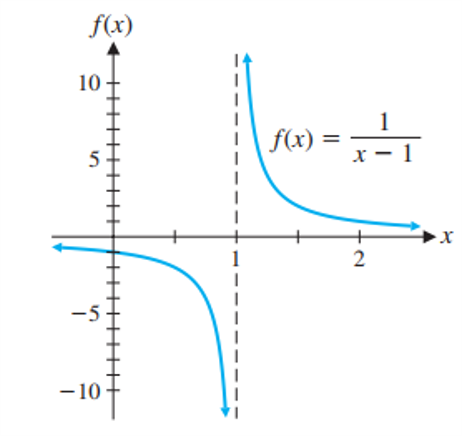
\includegraphics[width=0.5\textwidth]{9-2-20}
\end{center}
\begin{center}
	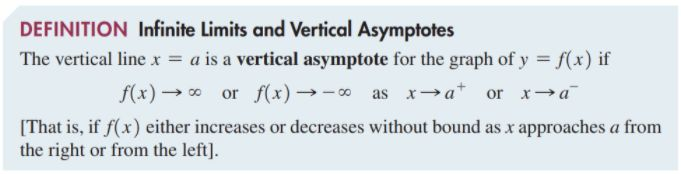
\includegraphics[width=0.9\textwidth]{9-2-20b}
\end{center}

\subsubsection{Locating Vertical Asymptotes}
\begin{itemize}
	\item Polynomial functions, $P(x)$, have no vertical asymptotes.
	\item Rational functions, ($R(x)=\frac{P(x)}{Q(x)}$), have a vertical asymptote whenever the numerator is not zero and the denominator is equal to 0.
	\item If both the numerator and the denominator of a rational function are zero, then we have an indeterminate form and more work must be done.
\end{itemize}
\begin{center}
	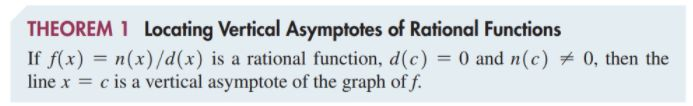
\includegraphics[width=0.9\textwidth]{9-2-20c}
\end{center}

\subsubsection{Example} Describe the behavior of f(x) at each zero of the denominator. Use $\infty$  or $-\infty$ when appropriate.
$$f(x) = \frac{x^2+x-2}{x^2-1}$$
We wish to find where the denominator equals zero. So, we start by factoring the denominator to get
$$f(x) = \frac{x^2+x-2}{(x+1)(x-1)}$$
Clearly, the denominator equals zero at $x=-1, x=1$. At $x=-1$, the numerator is $1-1-2=-2$ which is not zero. This tells us that a vertical asymptote exists at $x=-1$.

At $x=1$ however, the numerator is also equal to 0. So at $x=1$ $f(x)$ is indeterminate and more work must be done. Factor the numerator to get:
\begin{align*}
	\lim_{x\to 1}f(x) &=\lim_{x\to 1}\frac{(x+2)(x-1)}{(x+1)(x-1)} \\
	&=\lim_{x\to 1} \frac{(x+2)}{(x+1)} \\
	&= \frac{3}{2}
\end{align*}

\section{Limits at Infinity}
Limits at infinity and horizontal asymptotes are used to describe the behavior of functions as x assumes arbitrarily large positive values or arbitrarily large negative values. Limits at infinity are limits for either $x\to -\infty$ or $x\to \infty$.
\begin{center}
	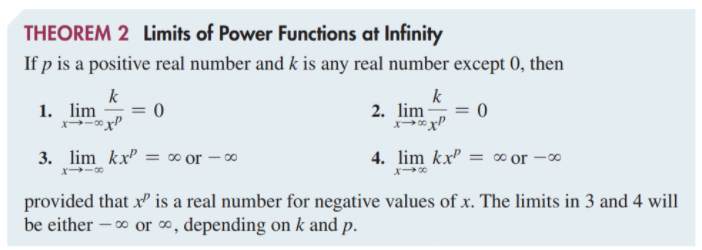
\includegraphics[width=0.9\textwidth]{9-2-5}
\end{center}
\begin{center}
	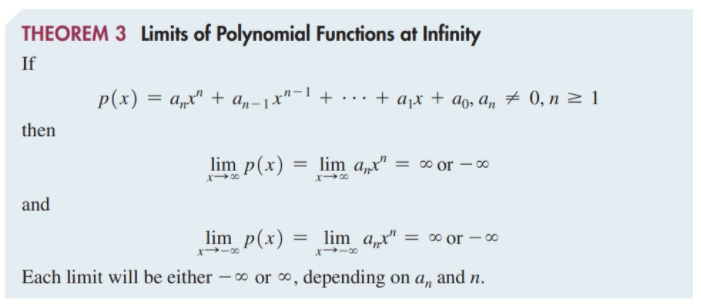
\includegraphics[width=0.9\textwidth]{9-2-6}
\end{center}

\subsection{Examples}
\begin{align*}
	&\lim_{x\to -\infty} \frac{20}{x^2}  = 0 \\
	&\lim_{x\to\infty} -38 x^4 = -\infty \\
	&\lim_{x\to\infty}(5x^3 -2x^2 -3x+6) = \lim_{x\to\infty}5x^3 = \infty
\end{align*}
A polynomial of degree 0 is a constant function $p(x) = a_0$, and its limit as $x\to \infty$ or $x\to -\infty$ is the number $a_0$. Polynomial functions of degree 1 or greater never have horizontal asymptotes.

\subsection{Horizontal Asymptotes}
\begin{center}
	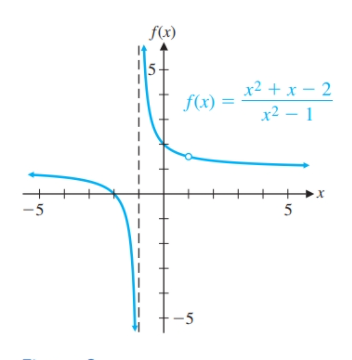
\includegraphics[width=0.4\linewidth]{9-2-1}
	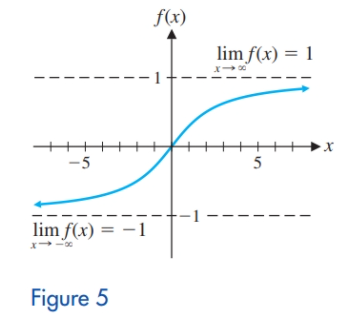
\includegraphics[width=0.4\linewidth]{9-2-4}
\end{center}
The horizontal asymptotes describe the end behavior of the function as $x\to -\infty$ and $x\to \infty$.

\begin{itemize}
	\item Some additional example graphs, \url{https://www.desmos.com/calculator/vshkxi2kdb}
\end{itemize}

\begin{center}
	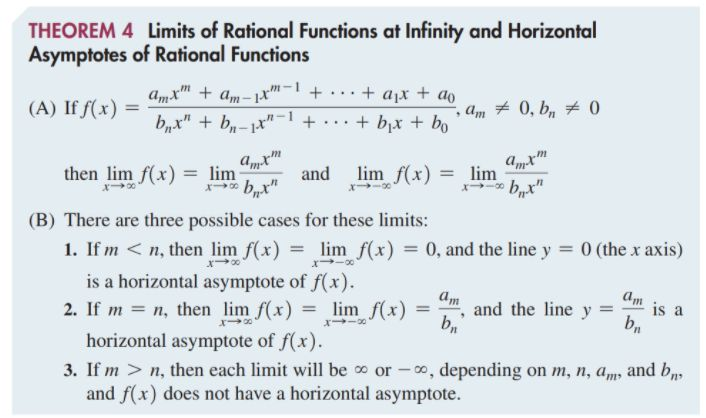
\includegraphics[width=1\textwidth]{9-2-20d}
\end{center}
\subsubsection{Examples}
Find the horizontal asymptotes and limits at infinity.
\begin{align*}
	\lim_{x\to -\infty} \frac{3x^4-5x^2 +2}{4x^3+2x+7} &= \lim_{x\to -\infty} \frac{3x^4}{4x^3} =
	\lim_{x\to -\infty} \frac{3x}{4} = -\infty \\\\
	\lim_{x\to \infty} \frac{3x^4-5x^2 +2}{4x^3+2x+7} &= \lim_{x\to \infty} \frac{3x^4}{4x^3} =
	\lim_{x\to \infty} \frac{3x}{4} = \infty
\end{align*}
This function has no horizontal asymptotes.

\begin{align*}
	\lim_{x\to -\infty} \frac{5x^3-2x^2 +2}{4x^4+7x+3} &= \lim_{x\to -\infty} \frac{5x^3}{4x^4} =
	\lim_{x\to -\infty} \frac{5}{4x} = 0 \\\\
	\lim_{x\to \infty} \frac{5x^3-2x^2 +2}{4x^4+7x+3} &= \lim_{x\to \infty} \frac{5x^3}{4x^4} =
	\lim_{x\to \infty} \frac{5}{4x} = 0
\end{align*}
This function has a horizontal asymptote at $y=0$

\begin{align*}
	\lim_{x\to -\infty} \frac{7x^3-10x^2 +4}{3x^3+9x-11} &= \lim_{x\to -\infty} \frac{7x^3}{3x^3} =
	\lim_{x\to -\infty} \frac{7}{3} = \frac{7}{3} \\\\
	\lim_{x\to \infty} \frac{7x^3-10x^2 +4}{3x^3+9x-11} &= \lim_{x\to \infty} \frac{7x^3}{3x^3} =
	\lim_{x\to \infty} \frac{7}{3} = \frac{7}{3} 
\end{align*}
This function has a horizontal asymptote at $y=\frac{7}{3}$




\noindent\rule{\textwidth}{1pt}
{\footnotesize Copyright (C) 2021 Garold Dalton --- Released under GNU General Public License v3.0}


\cleardoublepage


\end{document}
